\documentclass[a4paper,twoside]{article}
\usepackage{blindtext}  
\usepackage{geometry}

% Chinese support
\usepackage[UTF8, scheme = plain]{ctex}

% Page margin layout
\geometry{left=2.3cm,right=2cm,top=2.5cm,bottom=2.0cm}


\usepackage{listings}
\usepackage{xcolor}
\usepackage{geometry}
\usepackage{amsmath}
\usepackage{float}
\usepackage{hyperref}

\usepackage{graphics}
\usepackage{graphicx}
\usepackage{subfigure}
\usepackage{epsfig}
\usepackage{float}

\usepackage{algorithm}
\usepackage[noend]{algpseudocode}

\usepackage{booktabs}
\usepackage{threeparttable}
\usepackage{longtable}
\usepackage{listings}
\usepackage{tikz}
\usepackage{multicol}

% cite package, to clean up citations in the main text. Do not remove.
\usepackage{cite}

\usepackage{color,xcolor}

%% The amssymb package provides various useful mathematical symbols
\usepackage{amssymb}
%% The amsthm package provides extended theorem environments
\usepackage{amsthm}
\usepackage{amsfonts}
\usepackage{enumerate}
\usepackage{enumitem}
\usepackage{listings}

\usepackage{indentfirst}
\setlength{\parindent}{2em} % Make two letter space in the first paragraph
\usepackage{setspace}
\linespread{1.5} % Line spacing setting
\usepackage{siunitx}
\setlength{\parskip}{0.5em} % Paragraph spacing setting

% \usepackage[contents =22920202204622, scale = 10, color = black, angle = 50, opacity = .10]{background}

\renewcommand{\figurename}{图}
\renewcommand{\lstlistingname}{代码} 
\renewcommand{\tablename}{表格}
\renewcommand{\contentsname}{目录}
\floatname{algorithm}{算法}

\graphicspath{ {images/} }

%%%%%%%%%%%%%
\newcommand{\StudentNumber}{22920202204622}  % Fill your student number here
\newcommand{\StudentName}{熊恪峥}  % Replace your name here
\newcommand{\PaperTitle}{实验(一)}  % Change your paper title here
\newcommand{\PaperType}{Unix程序设计} % Replace the type of your report here
\newcommand{\Date}{2022年9月23日}
\newcommand{\College}{信息学院}
\newcommand{\CourseName}{Unix程序设计}
%%%%%%%%%%%%%

%% Page header and footer setting
\usepackage{fancyhdr}
\usepackage{lastpage}
\pagestyle{fancy}
\fancyhf{}
% This requires the document to be twoside
\fancyhead[LO]{\texttt{\StudentName }}
\fancyhead[LE]{\texttt{\StudentNumber}}
\fancyhead[C]{\texttt{\PaperTitle }}
\fancyhead[R]{\texttt{第{\thepage}页,共\pageref*{LastPage}页}}


\title{\PaperTitle}
\author{\StudentName}
\date{\Date}

\lstset{
	basicstyle          =   \sffamily,          % 基本代码风格
	keywordstyle        =   \bfseries,          % 关键字风格
	commentstyle        =   \rmfamily\itshape,  % 注释的风格,斜体
	stringstyle         =   \ttfamily,  % 字符串风格
	flexiblecolumns,                % 别问为什么,加上这个
	numbers             =   left,   % 行号的位置在左边
	showspaces          =   false,  % 是否显示空格,显示了有点乱,所以不现实了
	numberstyle         =   \zihao{-5}\ttfamily,    % 行号的样式,小五号,tt等宽字体
	showstringspaces    =   false,
	captionpos          =   t,      % 这段代码的名字所呈现的位置,t指的是top上面
	frame               =   lrtb,   % 显示边框
}

\lstdefinestyle{PythonStyle}{
	language        =   Python, % 语言选Python
	basicstyle      =   \zihao{-5}\ttfamily,
	numberstyle     =   \zihao{-5}\ttfamily,
	keywordstyle    =   \color{blue},
	keywordstyle    =   [2] \color{teal},
	stringstyle     =   \color{magenta},
	commentstyle    =   \color{red}\ttfamily,
	breaklines      =   true,   % 自动换行,建议不要写太长的行
	columns         =   fixed,  % 如果不加这一句,字间距就不固定,很丑,必须加
	basewidth       =   0.5em,
}

\lstdefinestyle{CppStyle}{
	language        =   c++,
	basicstyle      =   \zihao{-5}\ttfamily,
	numberstyle     =   \zihao{-5}\ttfamily,
	keywordstyle    =   \color{blue},
	keywordstyle    =   [2] \color{teal},
	stringstyle     =   \color{magenta},
	commentstyle    =   \color{red}\ttfamily,
	breaklines      =   true,   % 自动换行,建议不要写太长的行
	columns         =   fixed,  % 如果不加这一句,字间距就不固定,很丑,必须加
	basewidth       =   0.5em,
}

\algnewcommand\algorithmicinput{\textbf{Input:}}
\algnewcommand\algorithmicoutput{\textbf{Output:}}
\algnewcommand\Input{\item[\algorithmicinput]}%
\algnewcommand\Output{\item[\algorithmicoutput]}%

\usetikzlibrary{positioning, shapes.geometric}

\begin{document}
	
%%%%%%%%%%%%%%%%%%%%%%%%%%%%%%%%%%%%%%%%%%%%
\makeatletter % change default title style
\renewcommand*\maketitle{%
	\begin{center} 
		\bfseries  % title 
		{\LARGE \@title \par}  % LARGE typesetting
		\vskip 1em  %  margin 1em
		{\global\let\author\@empty}  % no author information
		{\global\let\date\@empty}  % no date
		\thispagestyle{empty}   %  empty page style
	\end{center}%
	\setcounter{footnote}{0}%
}
\makeatother
%%%%%%%%%%%%%%%%%%%%%%%%%%%%%%%%%%%%%%%%%%%%
	
	
\thispagestyle{empty}

\vspace*{1cm}

\begin{figure}[h]
	\centering
	
\includegraphics[width=4.0cm]{logo.png}
\end{figure}

\vspace*{1cm}

\begin{center}
	\Huge{\textbf{\PaperType}}
	
	\Large{\PaperTitle}
\end{center}

\vspace*{1cm}

\begin{table}[h]
	\centering	
	\begin{Large}
		\renewcommand{\arraystretch}{1.5}
		\begin{tabular}{p{3cm} p{5cm}<{\centering}}
			姓\qquad 名 & \StudentName  \\
			\hline
			学\qquad号 & \StudentNumber \\
			\hline
			日\qquad期 & \Date  \\
			\hline
			学\qquad院 & \College  \\
			\hline
			课程名称 & \CourseName  \\
			\hline
		\end{tabular}
	\end{Large}
\end{table}

\newpage

\title{
	\Large{\textcolor{black}{\PaperTitle}}
}
	
	
\maketitle
	
\tableofcontents
 
\newpage
\setcounter{page}{1}

\begin{spacing}{1.2}

\section{课件中讲到的每一个命令,都在命令行下试一下。}

\subsection{cat}

\begin{figure}[H]
	\centering
	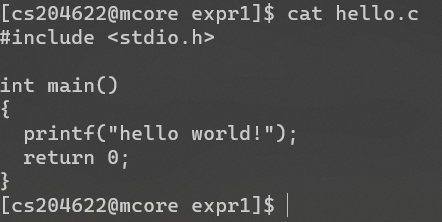
\includegraphics[width=8.0cm]{cat.png}
	\caption{cat}
\end{figure}

\subsection{cd和ls}

\begin{figure}[H]
	\centering
	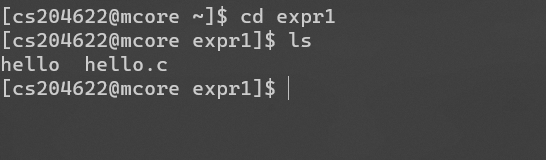
\includegraphics[width=8.0cm]{cdls.png}
	\caption{cd和ls}
\end{figure}

\subsection{cp}

\begin{figure}[H]
	\centering
	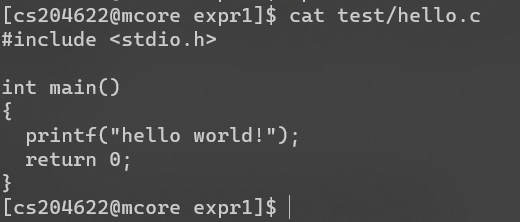
\includegraphics[width=8.0cm]{cp.png}
	\caption{cp}
\end{figure}

\subsection{diff}

\begin{figure}[H]
	\centering
	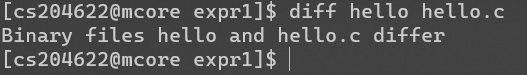
\includegraphics[width=8.0cm]{diff.png}
	\caption{diff}
\end{figure}

\subsection{find和grep}

\begin{figure}[H]
	\centering
	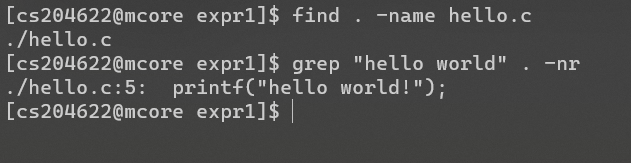
\includegraphics[width=8.0cm]{findgrep.png}
	\caption{find和grep}
\end{figure}

\subsection{man}

\begin{figure}[H]
	\centering
	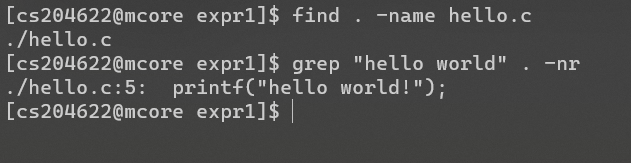
\includegraphics[width=8.0cm]{findgrep.png}
	\caption{man}
\end{figure}

\subsection{mv}

\begin{figure}[H]
	\centering
	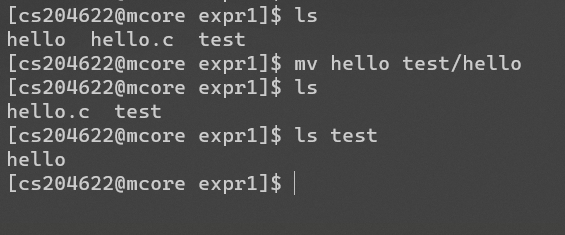
\includegraphics[width=8.0cm]{mv.png}
	\caption{mv}
\end{figure}

\subsection{ps}

\begin{figure}[H]
	\centering
	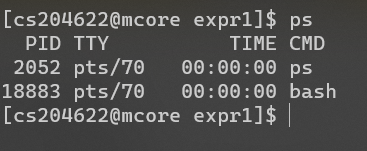
\includegraphics[width=8.0cm]{ps.png}
	\caption{ps}
\end{figure}

\subsection{pwd、mkdir和rmdir}

\begin{figure}[H]
	\centering
	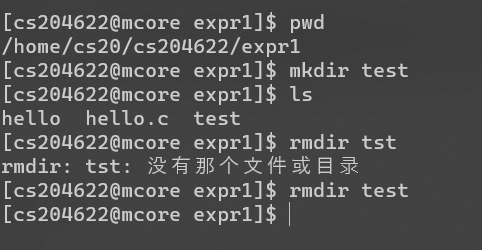
\includegraphics[width=8.0cm]{pwdmkdir.png}
	\caption{pwd、mkdir和rmdir}
\end{figure}

\subsection{who、whoami等}

\begin{figure}[H]
	\centering
	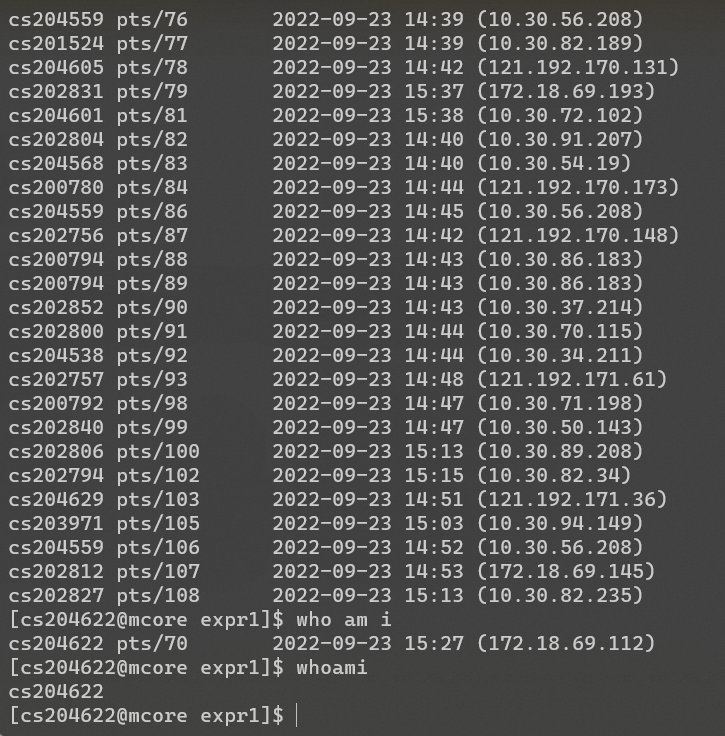
\includegraphics[width=8.0cm]{who.png}
	\caption{who、whoami等}
\end{figure}

\subsection{IO重定向}

\begin{figure}[H]
	\centering
	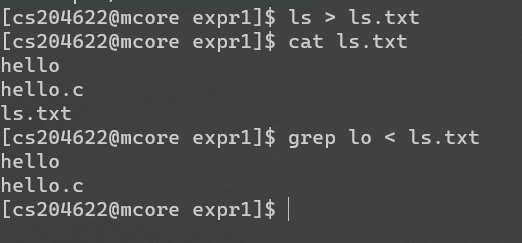
\includegraphics[width=8.0cm]{ioredir.png}
	\caption{find和grep}
\end{figure}

\clearpage

\section{编辑一个C语言文件,内容为ppt中的输出hello world的文件,保存为.c 文件,然后用gcc命令编译,执行编译后的文件并输出到屏幕。}

我认为nano编辑器比vi更好用。因此我用nano创建hello.c,并输入代码如图~\ref{fig:hello_code}。

\begin{figure}[htb]
	\centering
	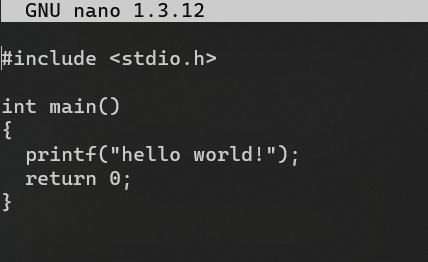
\includegraphics[width=6.0cm]{hello_code.png}
	\caption{代码}
	\label{fig:hello_code}
\end{figure}

然后使用gcc编译器编译并运行,如图~\ref{fig:cmp_run}。

\begin{figure}[htb]
	\centering
	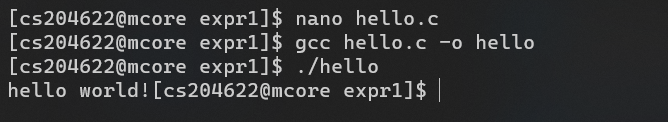
\includegraphics[width=8.0cm]{hello.png}
	\caption{代码}
	\label{fig:cmp_run}
\end{figure}

可见正常输出了hello world内容。

\section{利用ftp登录到unix服务器}

我使用sftp命令连接到服务器。首先按照\ref{sec:ssh}节中的方法配置ssh配置文件,然后在
控制台中输入\textbf{sftp -P 10022 cs204622@59.77.8.124},并按照提示输入密码。这样就可以
操作文件。如图~\ref{fig:sftp}。
\begin{figure}[htb]
	\centering
	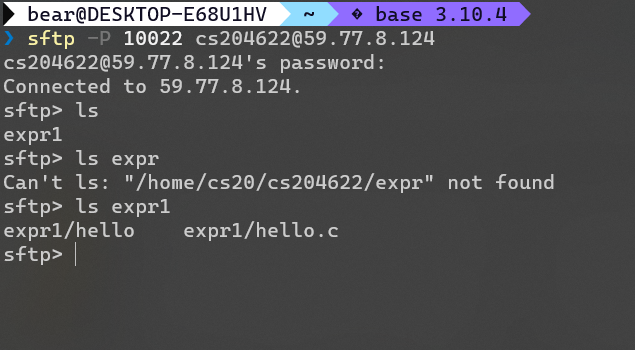
\includegraphics[width=8.0cm]{sftp.png}
	\caption{SFTP连接}
	\label{fig:sftp}
\end{figure}

\section{利用putty或者其他shell工具,登录服务器。}
\label{sec:ssh}

我直接使用ssh命令登录到服务器。首先,由于服务器的内核版本为2.6,它\emph{过于老旧}了。
因此为了解决\emph{落后的内核版本不支持新的加密标准的问题},需要先配置ssh工具。
如图~\ref{fig:sshconf}。
\begin{figure}[htb]
	\centering
	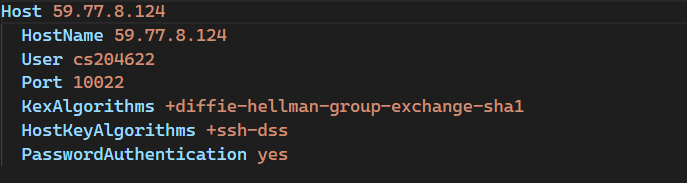
\includegraphics[width=8.0cm]{sshconf.png}
	\caption{配置SSH}
	\label{fig:sshconf}
\end{figure}
在Windows客户机的
\%USERPROFILE\%/.ssh/config中加入图~\ref{fig:sshconf}中的配置内容,其中前3行
配置了服务器地址、用户名和端口,第4、5行启用了一个该\emph{老旧服务器}支持的ssh加密算法,
最后一行启用了密码登录。

然后,在控制台中使用命令\textbf{ssh cs204622@59.77.8.124 -p 10022}登陆服务器。出现图~\ref{fig:ssh}
中的提示,按提示输入密码,登录到服务器,如图~\ref{fig:server}。

\begin{figure}[htb]
	\centering
	\begin{minipage}[t]{0.48\textwidth}
		\centering
		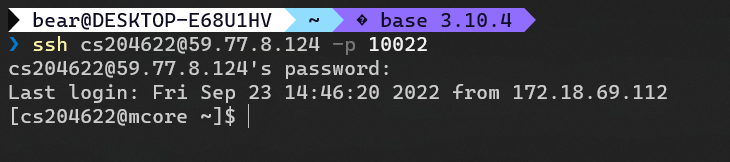
\includegraphics[width=6.0cm]{ssh.png}
		\caption{使用SSH登录到服务器}
		\label{fig:ssh}
	\end{minipage}
	\begin{minipage}[t]{0.48\textwidth}
		\centering
		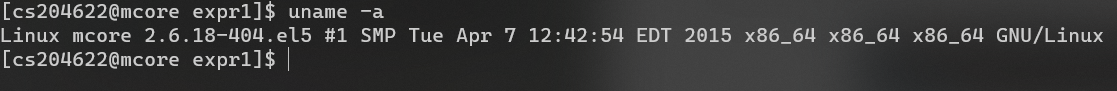
\includegraphics[width=8.0cm]{server.png}
		\caption{服务器内容}
		\label{fig:server}
	\end{minipage}
\end{figure}


\end{spacing}

\end{document}